% Options for packages loaded elsewhere
\PassOptionsToPackage{unicode}{hyperref}
\PassOptionsToPackage{hyphens}{url}
\PassOptionsToPackage{dvipsnames,svgnames,x11names}{xcolor}
%
\documentclass[
]{article}

\usepackage{amsmath,amssymb}
\usepackage{iftex}
\ifPDFTeX
  \usepackage[T1]{fontenc}
  \usepackage[utf8]{inputenc}
  \usepackage{textcomp} % provide euro and other symbols
\else % if luatex or xetex
  \usepackage{unicode-math}
  \defaultfontfeatures{Scale=MatchLowercase}
  \defaultfontfeatures[\rmfamily]{Ligatures=TeX,Scale=1}
\fi
\usepackage{lmodern}
\ifPDFTeX\else  
    % xetex/luatex font selection
  \setmainfont[]{Latin Modern Roman}
  \setmathfont[]{Latin Modern Math}
\fi
% Use upquote if available, for straight quotes in verbatim environments
\IfFileExists{upquote.sty}{\usepackage{upquote}}{}
\IfFileExists{microtype.sty}{% use microtype if available
  \usepackage[]{microtype}
  \UseMicrotypeSet[protrusion]{basicmath} % disable protrusion for tt fonts
}{}
\makeatletter
\@ifundefined{KOMAClassName}{% if non-KOMA class
  \IfFileExists{parskip.sty}{%
    \usepackage{parskip}
  }{% else
    \setlength{\parindent}{0pt}
    \setlength{\parskip}{6pt plus 2pt minus 1pt}}
}{% if KOMA class
  \KOMAoptions{parskip=half}}
\makeatother
\usepackage{xcolor}
\setlength{\emergencystretch}{3em} % prevent overfull lines
\setcounter{secnumdepth}{5}
% Make \paragraph and \subparagraph free-standing
\ifx\paragraph\undefined\else
  \let\oldparagraph\paragraph
  \renewcommand{\paragraph}[1]{\oldparagraph{#1}\mbox{}}
\fi
\ifx\subparagraph\undefined\else
  \let\oldsubparagraph\subparagraph
  \renewcommand{\subparagraph}[1]{\oldsubparagraph{#1}\mbox{}}
\fi


\providecommand{\tightlist}{%
  \setlength{\itemsep}{0pt}\setlength{\parskip}{0pt}}\usepackage{longtable,booktabs,array}
\usepackage{calc} % for calculating minipage widths
% Correct order of tables after \paragraph or \subparagraph
\usepackage{etoolbox}
\makeatletter
\patchcmd\longtable{\par}{\if@noskipsec\mbox{}\fi\par}{}{}
\makeatother
% Allow footnotes in longtable head/foot
\IfFileExists{footnotehyper.sty}{\usepackage{footnotehyper}}{\usepackage{footnote}}
\makesavenoteenv{longtable}
\usepackage{graphicx}
\makeatletter
\def\maxwidth{\ifdim\Gin@nat@width>\linewidth\linewidth\else\Gin@nat@width\fi}
\def\maxheight{\ifdim\Gin@nat@height>\textheight\textheight\else\Gin@nat@height\fi}
\makeatother
% Scale images if necessary, so that they will not overflow the page
% margins by default, and it is still possible to overwrite the defaults
% using explicit options in \includegraphics[width, height, ...]{}
\setkeys{Gin}{width=\maxwidth,height=\maxheight,keepaspectratio}
% Set default figure placement to htbp
\makeatletter
\def\fps@figure{htbp}
\makeatother

\usepackage{arxiv}
\usepackage{orcidlink}
\usepackage{amsmath}
\usepackage[T1]{fontenc}
\makeatletter
\@ifpackageloaded{caption}{}{\usepackage{caption}}
\AtBeginDocument{%
\ifdefined\contentsname
  \renewcommand*\contentsname{Table of contents}
\else
  \newcommand\contentsname{Table of contents}
\fi
\ifdefined\listfigurename
  \renewcommand*\listfigurename{List of Figures}
\else
  \newcommand\listfigurename{List of Figures}
\fi
\ifdefined\listtablename
  \renewcommand*\listtablename{List of Tables}
\else
  \newcommand\listtablename{List of Tables}
\fi
\ifdefined\figurename
  \renewcommand*\figurename{Figure}
\else
  \newcommand\figurename{Figure}
\fi
\ifdefined\tablename
  \renewcommand*\tablename{Table}
\else
  \newcommand\tablename{Table}
\fi
}
\@ifpackageloaded{float}{}{\usepackage{float}}
\floatstyle{ruled}
\@ifundefined{c@chapter}{\newfloat{codelisting}{h}{lop}}{\newfloat{codelisting}{h}{lop}[chapter]}
\floatname{codelisting}{Listing}
\newcommand*\listoflistings{\listof{codelisting}{List of Listings}}
\makeatother
\makeatletter
\makeatother
\makeatletter
\@ifpackageloaded{caption}{}{\usepackage{caption}}
\@ifpackageloaded{subcaption}{}{\usepackage{subcaption}}
\makeatother
\ifLuaTeX
  \usepackage{selnolig}  % disable illegal ligatures
\fi
\usepackage{bookmark}

\IfFileExists{xurl.sty}{\usepackage{xurl}}{} % add URL line breaks if available
\urlstyle{same} % disable monospaced font for URLs
\hypersetup{
  pdftitle={The Positive Relationship of Walkability on Diabetes Prevalence in the Southern United States},
  pdfauthor={Arkaprabho Bose; Sebastian Oberg; Abhinav Cheruvu},
  colorlinks=true,
  linkcolor={blue},
  filecolor={Maroon},
  citecolor={Blue},
  urlcolor={Blue},
  pdfcreator={LaTeX via pandoc}}

\usepackage{lineno}
\linenumbers
\usepackage{setspace}
\doublespacing
\newcommand{\runninghead}{A Preprint }
\renewcommand{\runninghead}{A Preprint }
\title{The Positive Relationship of Walkability on Diabetes Prevalence
in the Southern United States}
\def\asep{\\\\\\ } % default: all authors on same column
\author{\textbf{Arkaprabho Bose}\\Undergraduate Program in Department of
Computer Science\\Texas A \& M University\\College Station,
TX,\ 77843\\\href{mailto:abose0267@tamu.edu}{abose0267@tamu.edu}\asep\textbf{Sebastian
Oberg}\\Undergraduate Program in Department of Computer Science\\Texas A
\& M University\\College Station, TX,\ 77843\\\asep\textbf{Abhinav
Cheruvu}\\Undergraduate Program in Department of Mathematics\\Texas A \&
M University\\College Station, TX,\ 77843\\}
\date{}
\begin{document}
\maketitle
\begin{abstract}
The diabetes epidemic in the United States presents a nuanced public
health challenge, shaped by factors such as socioeconomic status and
climate. While the influence of these factors on diabetes is
well-established, the role of walkability in managing diabetes
prevalence remains contested. This study revisits the relationship
between walkability and diabetes in the U.S., using walkability indexes
calculated from CDC data. Contrary to some studies suggesting that
increased walkability reduces diabetes prevalence, our findings,
analyzed through Geographically Weighted Regression (GWR), reveal that
walkability is not a significant predictor of diabetes prevalence and
exhibits notable regional anomalies. Further analysis using Monte Carlo
simulations, Global I Moran's Test, and Variance Inflation Ratio (VIR)
supports these results. Our study also critiques the current methods of
calculating the walkability index, proposing a revised model that
incorporates additional relevant variables from the CDC. This nuanced
understanding underscores the need for region-specific urban planning
and public health strategies that recognize the complex interplay
between walkability, environmental, and socioeconomic factors.
\end{abstract}

\section{Introduction}\label{sec-intro}

Diabetes is a common chronic illness that is caused due to consistently
high blood sugar levels, and can be prevented through sugar intake
management, exercise and dieting. In a study done on 2016 and 2017
National Center for Health Statistics data, it was shown that among
adults in the United States, there was a prevalence of 9.7\% (Xu, et.
al). This high prevalence can impact humans on a daily basis by directly
impacting the quality of life both physically and mentally. Diabetes can
affect organs all around the body such as the eyes, pancreas and
kidneys. In addition to having direct impact on people, high prevalence
of diabetes puts stress on the existing healthcare systems by forcing
hospitals and doctors to put resources into solving issues that are
preventable.

In recent years, there have been speculations that lifestyle changes,
specifically walkability of a region can impact the prevalence of
diabetes in that given region. The Environmental Protection Agency has
developed a standardized scale on which regions can be ranked based on
how walkable it is. The scale ranges from 1-20 with 1 being the least
walkable and 20 being the most walkable. It takes into account various
things such as intersection density, and proximity to transit (Glazier
et al.). According to a temporal analysis study done in 2016, areas with
highest walkability score, which is a value calculated had lower rates
of diabetes prevalence (Creatore et. al). An area being walkable results
in less reliance on cars, and forces the population to walk which is a
form of exercise that is often overlooked and can have a meaningful
impact on ones health.

As of right now, there is no global standard for calculating something
like a walkability index score. This leads to different organizations
and institutions coming up with their own, and causing discrepancies in
their results. As we will discuss later in the article, the United
States standard for walkability index is created by the Environmental
Protection Agency. If this really is being used at a government level as
the standard, it is important for the methodology they use to calculate
their scores to be thoroughly investigated to see if it is truly
representative of a places walkability, and whether there are ways to
improve their model.

It is crucial to understand the availability index, so that the correct
actions can be taken to decrease the prevalence of diabetes in the
necessary regions. If regions are showing increase in disease
prevalence, and their walkability index is showing it to be incorrect,
then people like urban planners will not take the necessary steps to
solve the issues.

\section{Related Works}\label{related-works}

\subsection{Significance of Walkability on Diabetes
Prevalence}\label{significance-of-walkability-on-diabetes-prevalence}

The study ``Walkability and its association with prevalent and incident
diabetes in a pooled sample from five German cohorts'' highlights the
crucial impact of walkability on diabetes prevalence. By integrating
Geographically Weighted Regression (GWR) to analyze the relationship
between neighborhood walkability and diabetes across Germany, the study
finds that higher walkability scores are generally associated with lower
rates of diabetes. This supports our hypothesis that improving
walkability in U.S. counties could serve as an effective preventive
measure against diabetes. These findings are directly applicable to our
research, which suggests that enhancements in urban design that
prioritize walkability could significantly contribute to public health
improvements.

\subsection{Comparative Analysis with Similar
Research}\label{comparative-analysis-with-similar-research}

The study ``Neighborhood walkability and pre-diabetes incidence in a
multiethnic population'' provides a significant comparative analysis to
our work. It examines the potential of walkable neighborhoods to
mitigate early stages of diabetes, using a comprehensive dataset from
Southern Ontario, Canada. The use of GWR to map spatial variances in
pre-diabetes incidence reveals that walkability can significantly
influence diabetes management across diverse populations. This parallels
our findings and methodological approach, which emphasizes the
importance of considering ethnic and demographic factors when assessing
the health impacts of urban walkability.

\subsection{Understanding the EPA's National Walkability
Index}\label{understanding-the-epas-national-walkability-index}

The ``National Walkability Index'' developed by the Environmental
Protection Agency (EPA) is a comprehensive tool for assessing
walkability across the United States. These variables include:

\begin{enumerate}
\def\labelenumi{\arabic{enumi}.}
\item
  \textbf{Intersection Density}: Measures the potential connectivity of
  pedestrian paths by calculating the number of intersections per square
  kilometer. High intersection density generally indicates more walkable
  areas as it suggests greater connectivity and options for pedestrian
  movement.
\item
  \textbf{Proximity to Transit Stops}: Evaluates the accessibility of
  public transit by measuring the distance from the population center of
  a block group to the nearest transit stop. Closer proximity implies
  better walkability as it eases access to public transportation.
\item
  \textbf{Employment Mix}: Assesses the diversity of job types within a
  walking distance. A diverse employment mix within close proximity can
  enhance walkability by reducing the need for long commutes and
  encouraging walking to work.
\item
  \textbf{Employment and Household Mix}: Analyzes the balance between
  residential locations and job locations. An optimal mix promotes
  walking by enabling residents to live closer to where they work, which
  promotes a walkable environment.
\end{enumerate}

By using these variables, the EPA's index not only measures the physical
infrastructure that supports walking but also considers how these
elements interact with socio-economic factors to affect public health
outcomes positively.

\subsection{Variations in Walkability Index
Methodologies}\label{variations-in-walkability-index-methodologies}

In the study ``Development of an objectively measured walkability index
for the Netherlands,'' a methodology is used that differs from the EPA's
approach. This method uses circular buffers, which are zones around a
given point, usually the geographic center of a postal code area, to
measure how many important amenities are within walking distance. These
buffers help in accurately assessing the accessibility of essential
services like groceries, parks, and schools, which are significant for
day-to-day living. A tailored approach like this highlights the
importance of considering localized settings and cultural norms in
walkability assessments to ensure that the indices are reflective of the
actual conditions experienced by residents.

\subsection{Comparative Approaches to Walkability
Assessments}\label{comparative-approaches-to-walkability-assessments}

In ``Planning and Design Support Tools for Walkability,'' the study
pieces walkability into categories such as transport and land use, which
examines the infrastructural and spatial arrangements that facilitate
walking; urban health, focusing on how walkable environments affect
physical and mental well-being; and livable cities, which looks at the
overall quality of life in urban settings. Each category uses different
analytical tools, from spatial analysis by means of Geographic
Information Systems (GIS) for detailed mapping, to qualitative methods
like surveys to gather resident experiences. This diverse methodology
provides urban analysts with robust tools for specific applications and
supports comprehensive urban planning that fosters sustainable and
healthy communities.

\subsection{Innovations in Walkability Index
Calculations}\label{innovations-in-walkability-index-calculations}

The study ``Spatial Pattern of the Walkability Index, Walk Score and
Walk Score Modification for Elderly'' highlight innovative adaptations
of common walkability indices to better cater to the elderly. This
adaptation considers factors like gait speed and proximity to
age-appropriate facilities, altering traditional indices to reflect the
mobility and access needs of older adults. These considerations are
important for creating inclusive urban environments that support the
independence and health of all citizens, especially as demographic
profiles shift towards older populations.

\subsection{Context-Specific Walkability
Indices}\label{context-specific-walkability-indices}

The ``Development of a Child-Focused Walkability Index'' introduces a
specialized approach by highlighting features like traffic volume and
the availability of sidewalks. These factors are significant in ensuring
that children have safe routes for school and recreational activities,
which promotes physical activity from a young age. By focusing on the
specific needs of children, this index highlights the necessity for
planning urban spaces that cater to the youngest residents, ensuring
their safety and well-being in city environments.

\section{Methods}\label{methods}

\subsection{Data}\label{data}

\subsubsection{Walkability Index}\label{walkability-index}

Walkability Index is a measurement of relative walkability that is
developed and calculated by the Environmental Protection Agency. The
goal of this measurement is to analyze different parts of the United
States on a common scale, and see trends related to walkability. The
Environmental Protection Agency calculates this walkability on a scale
1-20 with 1 being the least walkable, and 20 being the most. The actual
value on the walkability index scale is calculated using a few different
metrics that the EPA collects. The formula used is

\[\text{Walkability Index} = \frac{w}{3} + \frac{x}{3} +\frac{y}{6} + \frac{z}{6} \]

\begin{itemize}
\item
  \(w\) is a block group's intersection density, which is calculated by
  analyzing the number of different types of intersections.
  Intersections were defined by the types of roads the they connect. The
  types of road were defined as

  \begin{itemize}
  \item
    Auto Oriented: This type of road includes all roads that are geared
    for automotive use. Examples of this type of road includes highways
    and tollways where you would not expect pedestrians or bicyclists.
  \item
    Multi-Modal: Roads that are designed so that both automotive and
    pedestrians can simultaneously use it. This would include roads with
    separate bike lanes, and roads that fall under a certain speed limit
    depending on whether the road is one-way or two-way
  \item
    Pedestrian Oriented: Roads that are made primarily for pedestrian
    use, this can include neighborhood roads, and even paths and trails
    that auto-motives are not permitted on.
  \end{itemize}

  Based on these road types, intersection densities were calculated
  based on what types of road any given intersection is connecting. Once
  these intersection densities are calculated, an overall intersection
  density for the block group is calculated using a weighted sum of the
  components. This weighted sum penalizes intersections that are
  barriers for pedestrians. For example, intersections that connect two
  auto roads were given a weight of zero since it is expected to have
  little to no pedestrians. Similarly intersections connecting
  pedestrian oriented roads were given a high weight since it is
  expected to encourage and be easy for pedestrians to use
\item
  \(x\) is a measurement of the distance to the closest transit stop in
  meters. Specifically, geoprocessing models were used to calculate the
  distance from the block group centroid to the nearest transit stop.
  This value can directly impact walkability since people who live in
  places with higher walkability tend to rely less on cars and more on
  public transport whether it's by bus or train.
\item
  \(y\) is a block group's employment density mix. This is a variable
  that calculates the entropy of a block group based on the different
  jobs that are available in a certain area. This is one of the chosen
  factors for calculating walkability index since it takes into account
  the diversity of the area. In this case, a higher entropy would
  indicate a more diverse distribution of employment groups in the block
  group. The idea is that it will be a highly walkable place if there is
  a lot of different types of stores and businesses.
\item
  \(z\) is a block group's employment and household mix. This is a
  measurement of the diversity in a given region, in terms of businesses
  and occupied housing. Similar to the employment density mix, this
  measurement uses the entropy of businesses and housing to calculate an
  overall entropy value. This can be used to calculate a walkability
  score since it implies that with businesses and homes being close
  together, it is not necessary for employees to take a car to get to
  work, but rather take a form of public transit.
\end{itemize}

\emph{All formulas and variables were derived from the Environmental
Protection Agency Smart Location Database(Chapman et. al, 2021)}

\subsubsection{Other Covariates}\label{other-covariates}

In addition to walkability, we felt it was important to account for a
few different variables when conducting our study. We decided that based
on our research, it would be important to take into account several
different health factors that can impact diabetes prevalence. According
to an article by Mokdad et. al, there is a strong association between
diabetes and obesity, and obesity is tied into several other health
risks such as high blood pressure, and low physical activity. As a
response to this research, we decided to take common health issues into
account as covariates for our model. The health complications that we
focused on was the obesity, high blood pressure, smoking prevalence, and
low-physical activity. All of the chosen factors have some sort of
researched impact on diabetes prevalence and will allow for more
thorough results. In addition to this, we took into account the median
household income for all of the counties that we were working with, as
well as the average temperature. The health factors data was provided by
the CDC as part of their annual report (Center for Disease Control and
Prevention, 2023), and the median household income data was provided by
the United States Census Bureau, as part of their Small Area Income and
Poverty Estimates Program (United States Census Bureau, 2022). The
average temperature data was found from the GIS for Racial Equity
Website (Gilbert, 2023). Together these values will help lead to our
model fitting to be more complete and allow for more of the data to be
explained by the model.

\subsubsection{Data Cleaning}\label{data-cleaning}

Originally, we had started working with 4 different datasets, which we
then had to aggregate into one large dataset. The datasets had a lot of
data since most came from annual government reports, so it was important
to select only the relevant ones which were the spatial information and
the chosen covariates. Each of the datasets that we had decided to use
had originally been at the block group level. This was an issue as it
led to at least one value of relevant data being missing in some block
groups. Our solution for this issue was to average out the relevant
columns from each dataset at the county level. This took care of the
missing values as if one block group in a county was missing data, it
was dropped from the calculation and there were other block groups which
could be used as part of the average.

\subsection{Analysis}\label{analysis}

\subsubsection{Correlation Matrix}\label{correlation-matrix}

In order to get a general understanding of the data at hand, we
generated a correlation matrix to see the relationships between each of
the variables. This was also used as an exploratory tool to see if there
was any multicollinearity within our data. In the case of our project,
we used a threshold of 0.8 to find variables with concerning
similarities, and depending on the values in the correlation matrix,
conducted further analysis to ensure that the values that were highly
correlated were not impacting the results of the model heavily.

\subsubsection{Spatial Analysis}\label{spatial-analysis}

Based on the type of the data that was available, we chose to do spatial
analysis because we believed it would yield the best result. The model
we used in this study was Geographically Weighted Regression.
Specifically, we used the model provided by the GWModel Package (Gollini
et. al, 2015). This model, originally created by Brunsdon, is based on
the formula

\[y_i = \alpha_{0} + \sum_{k=1}^{m} \alpha_{k}x_{ik} + \varepsilon_{i}\]

\begin{itemize}
\tightlist
\item
  In the case of this formula:

  \begin{itemize}
  \tightlist
  \item
    \(y_i\) is the \(i\)th observation of the dependent variable
  \item
    \(\alpha_0\) is the intercept
  \item
    \(x_{ik}\) is the \(i\)th observation of the \(k\)th independent
    variable
  \item
    \(\varepsilon_{i}\) is the normally distributed independent error
    terms
  \item
    \(\alpha_{k}\) is estimated from \(n\) observations
  \end{itemize}
\end{itemize}

This model was chosen for this specific problem because it is able to
improve on regular regression models like global regression, and account
for spatial heterogeneity. In the case of our data, county level data
exhibits spatial heterogeneity due to how small the counties are
relative to the size of the United States. Initially, we had wondered
whether it would make sense to use this model in a predictive context,
but eventually decided that in order to investigate the relationship of
walkability on the diabetes prevalence, it would make more sense to use
the model in an inferential context. The GWModel package allowed for us
to set a formula where we set the diabetes prevalence as the response
variable and the covariates as the independent variables. The package
provides a function that, based on the inputted data identifies an ideal
bandwidth to use for the model. This bandwidth can then be used to fit
the model. Once the model was fit, it was important to adjust the
P-values to deal with insignificant coefficients to make the
visualization of the results more intuitive. Using the GWModel package,
the p-values were adjusted using the Fotheringham-Byrne procedures
(Gollini et. al,2015). Once this process was completed, coefficients
that had a significance level greater than 0.05 were zeroed out for
plotting purposes to show only the statistically significant
coefficients in the impact plot.

\subsubsection{Impact Plots}\label{impact-plots}

Once the insignificant coefficients were set to 0, we wanted to
understand how each covariate impacted the fitted diabetes prevalence
value in the GWR model. In order to do this, we used the original
observed diabetes data for each county, and multiplied it by the
predicted coefficients. It is important to note that since we adjusted
the P-values, there were a lot of cases where the impact was calculated
as 0 due to the adjusted coefficient. Once this calculation was done, it
was plotted spatially. Once these plots were made, we were able to make
inferences about the walkability index and it's relationship to
diabetes.

\subsection{Validation}\label{validation}

\subsubsection{Simulation Study}\label{simulation-study}

We conducted a simulation study to ensure that the model we had chosen
was truly a good model to fit on our type of data, and was not a random
fluke due to specific values. We conducted the simulation study by using
the original dataset along with spatially varying functions. The goal
here was to create realistic spatially varying coefficients for each
county, and that would be considered the ``true'' coefficient. The
coefficients were generated using a method that we wrote, which accepts
the latitude and longitude of a location, and generates realistic
coefficients for each covariate with both the longitude and latitude
being part of the calculation. This means that as each county's spatial
area changes, the impact of that covariate will change proportionally to
the distance. Once these ``true'' coefficients were calculated, we
calculated our ``true'' diabetes prevalence which was done by summing
the products of the ``true'' coefficient and the observed value for that
county. This ``true'' diabetes prevalence was then passed into a GWR
model as the response with the original observed values as the
independent variables. Success of this model was measured using the
adjusted R\^{}2 values, as well as a mean absolute error plot of the
``true'' coefficients and the predicted coefficients

\subsubsection{Diagnostics}\label{diagnostics}

In addition to the simulation study, we also ran a few different tests
to not only verify the validity of our model, but also as a way to
investigate why some of our results looked the way they did. The first
test that we ran was a Monte Carlo simulation on the residuals of our
model. The Monte Carlo simulation is conducted to identify which
variables are statistically significant. We analyzed the p-values to see
which of the chosen covariates are significantly spatially varying to
see if any of the covariates used could have been left out. In addition
to this, we used a Moran's I Test as a way to test for spatial
autocorrelation.

\section{Results}\label{results}

\subsection{Simulation Study using Artificial
Data}\label{simulation-study-using-artificial-data}

From the simulation study using artificial data, we obtained results
that demonstrate the strength of our GWR model. Our results depicted
below provide valid estimates and coefficients when fitting a GWR on our
simulated data. In our simulation study, the Mean Absolute Error ranged
from -1.63 to 0.05, which was fairly close to zero for each covariate.
This suggests the validity of our GWR model. Additionally, we obtained a
relatively high R-squared value of 0.94 when fitting a GWR model on our
artificial data, demonstrating strong explanatory power. Lastly, Plot 2
depicted below illustrates evenly dispersed residuals across the United
States, confirming the validity of our GWR model.

\begin{figure}[H]

{\centering 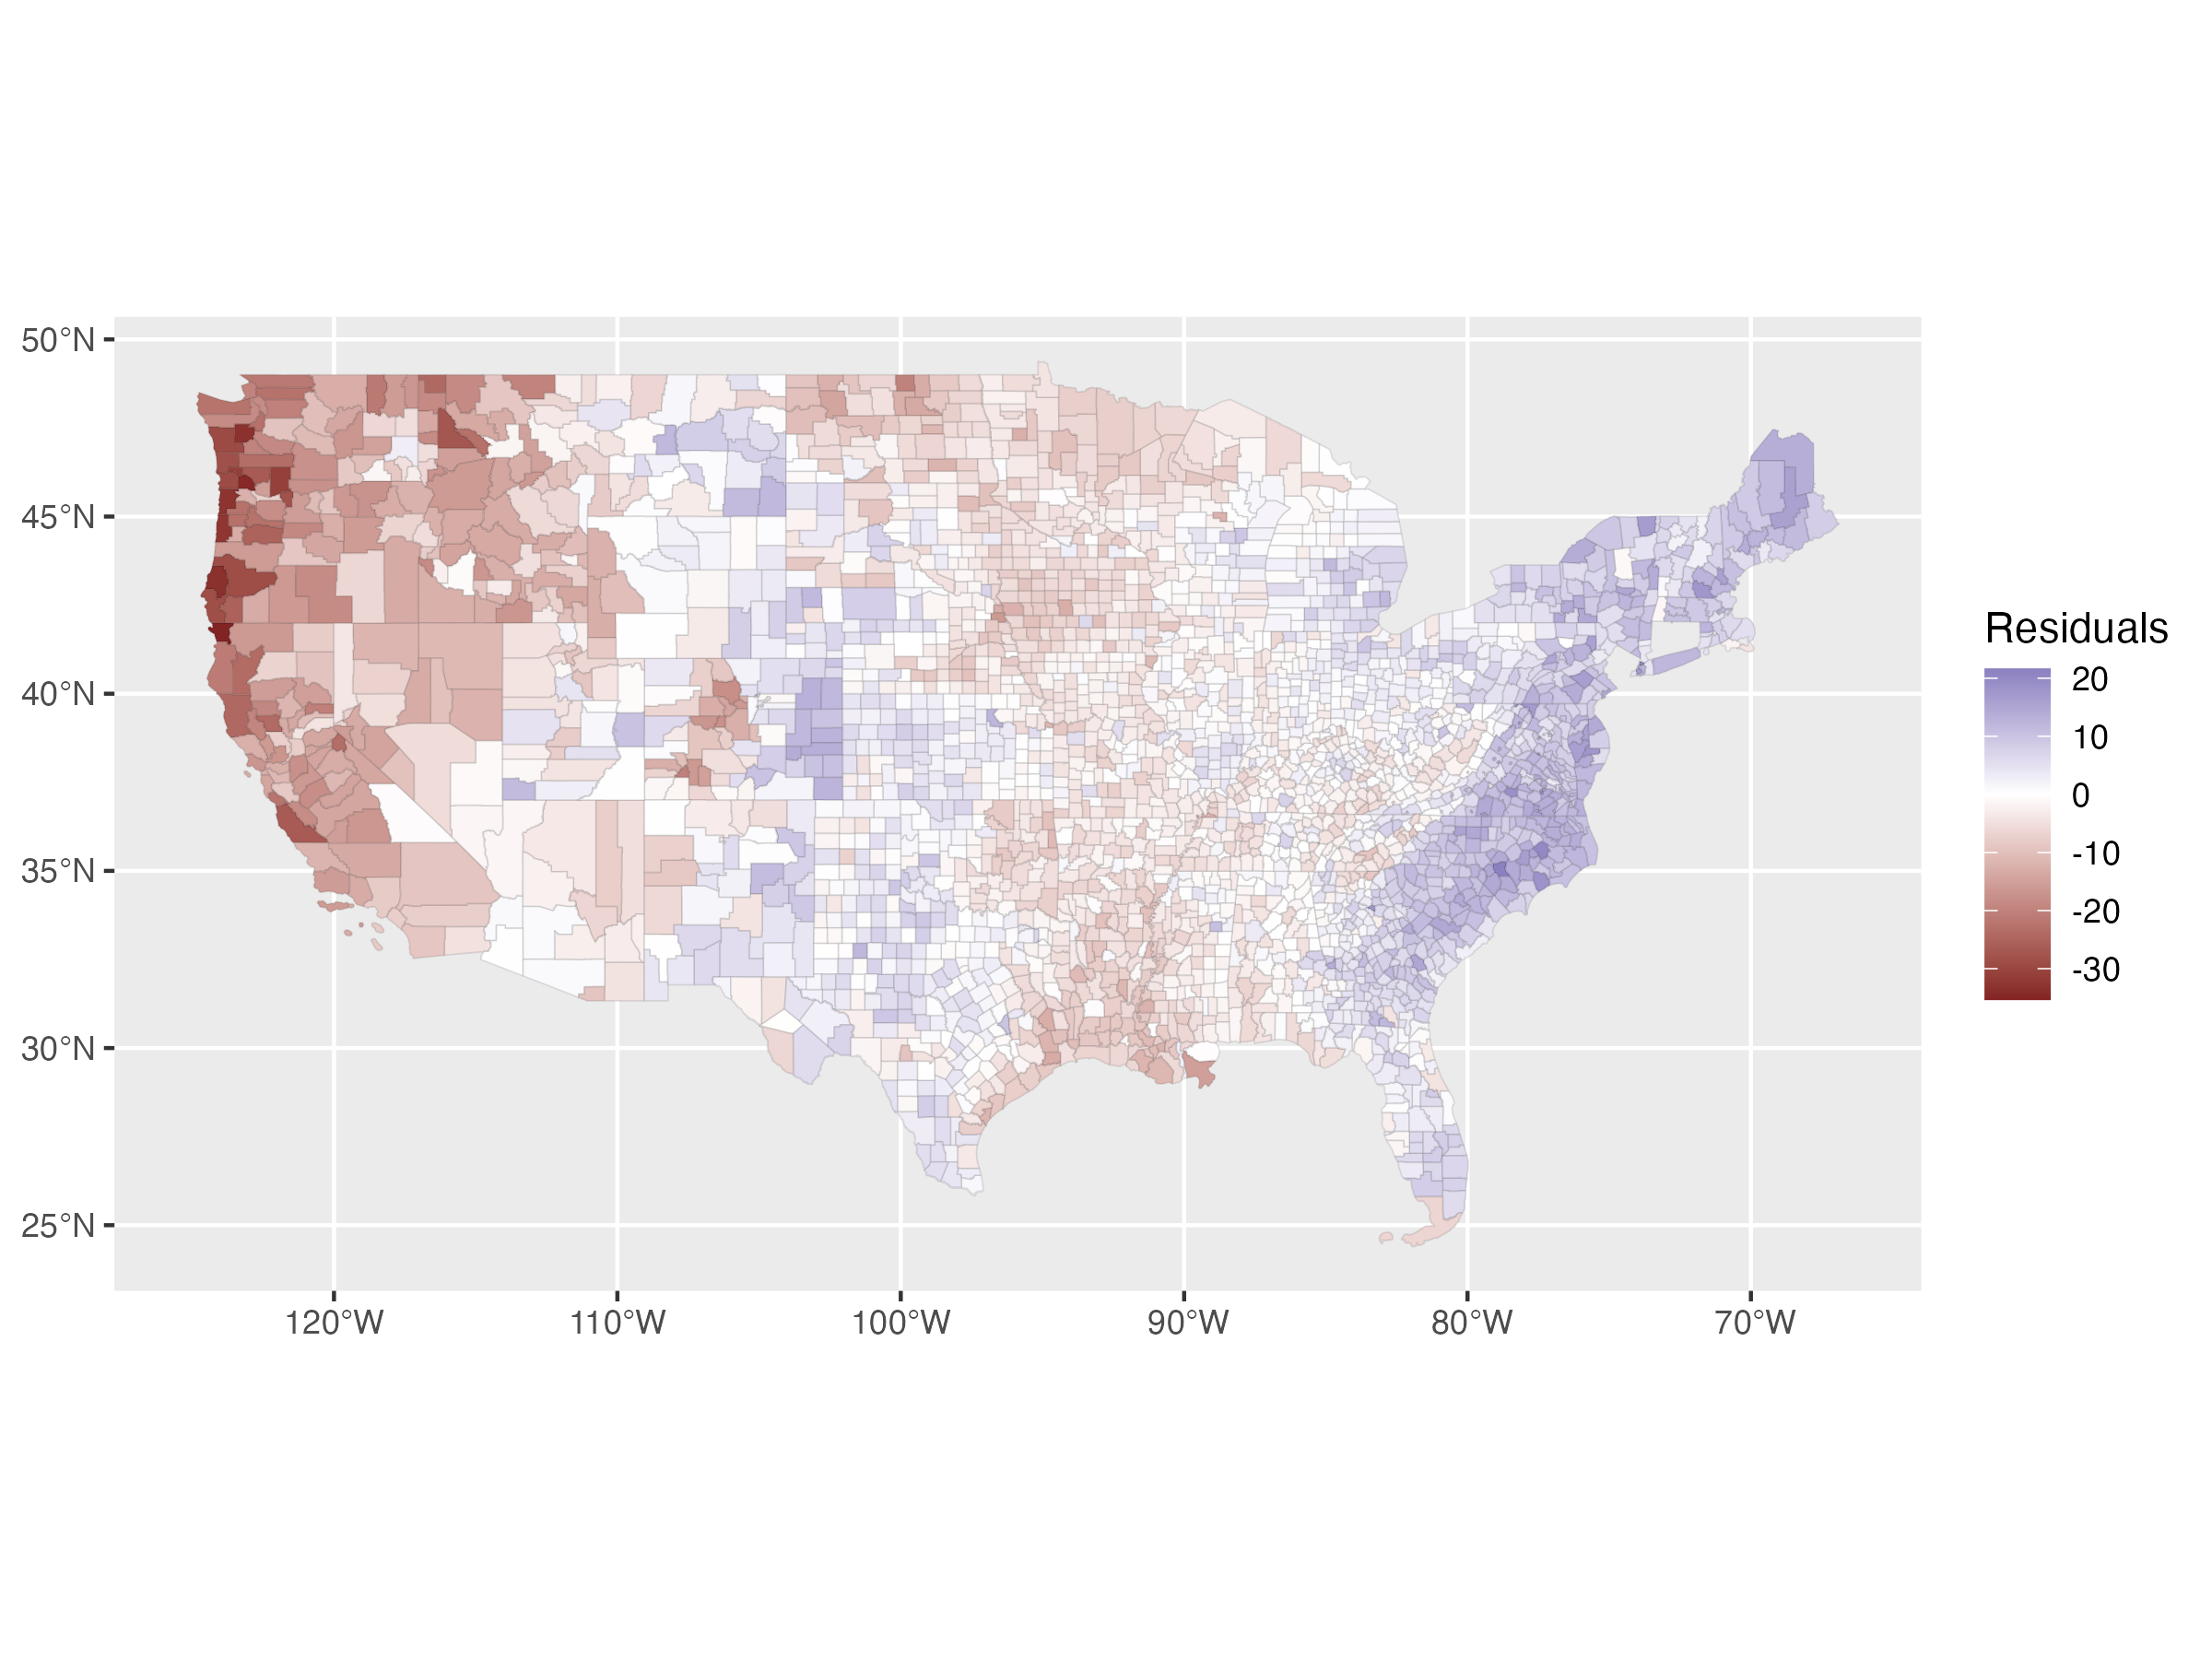
\includegraphics{sim_residual_plot.png}

}

\caption{Normalized Residuals of GWR Model Results on Simulated Data}

\end{figure}%

\begin{longtable}[]{@{}
  >{\raggedright\arraybackslash}p{(\columnwidth - 2\tabcolsep) * \real{0.5571}}
  >{\raggedleft\arraybackslash}p{(\columnwidth - 2\tabcolsep) * \real{0.4429}}@{}}
\caption{Mean Absolute Error of Coefficient Predictions for Simulated
Data}\tabularnewline
\toprule\noalign{}
\begin{minipage}[b]{\linewidth}\raggedright
Covariates
\end{minipage} & \begin{minipage}[b]{\linewidth}\raggedleft
Normalized Mean Absolute Error
\end{minipage} \\
\midrule\noalign{}
\endfirsthead
\toprule\noalign{}
\begin{minipage}[b]{\linewidth}\raggedright
Covariates
\end{minipage} & \begin{minipage}[b]{\linewidth}\raggedleft
Normalized Mean Absolute Error
\end{minipage} \\
\midrule\noalign{}
\endhead
\bottomrule\noalign{}
\endlastfoot
National Walkability Index & 1.6548125 \\
Obesity Crude Prevalence & 0.1453355 \\
High Blood Pressure Crude Prevalence & 0.2334461 \\
Low Physical Activity Crude Prevalence & 0.5575400 \\
Smoking Crude Prevalence & 0.7625102 \\
Average Temperature & 1.1054633 \\
Median Household Income & 17.0318290 \\
\end{longtable}

\subsection{Correlation Matrix}\label{correlation-matrix-1}

\begin{figure}[H]

{\centering 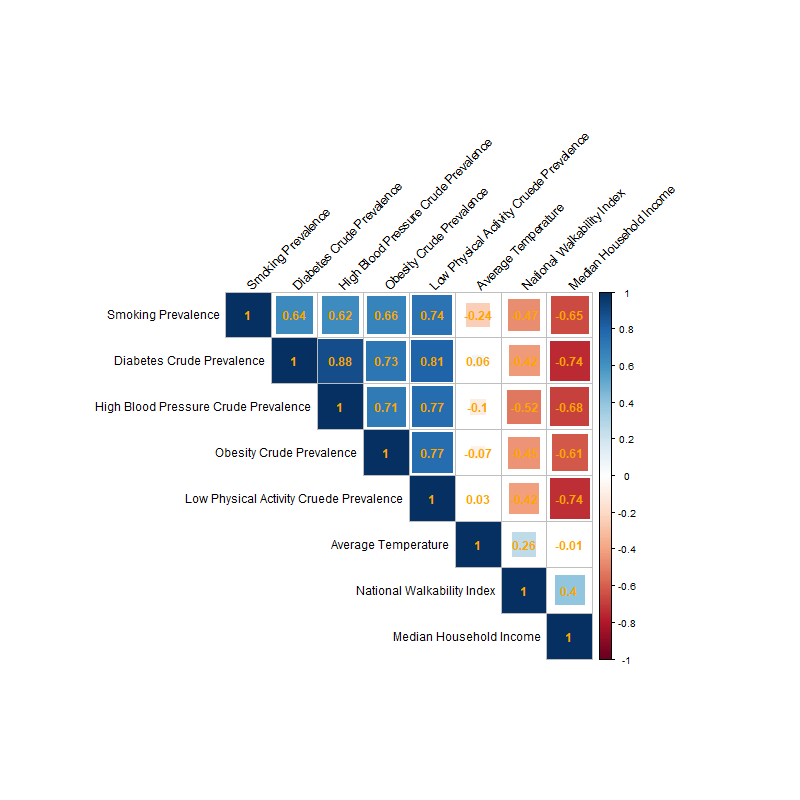
\includegraphics{correlation_plot.png}

}

\caption{Correlation Matrix of Chosen Variables}

\end{figure}%

From the Analysis of our Correlation Matrix plot above, we observed
several factors highly correlated with Diabetes Prevalence, notably High
Blood Pressure (correlation of 0.89) and Obesity (correlation of 0.74).
These health risk factors were incorporated into our model, providing
valuable insights into the multifaceted nature of diabetes prevalence
and its associated risks. While these factors demonstrate strong
positive associations, other covariates such as Average Temperature
(correlation of 0.01) and National Walkability Index (correlation of
-0.44) were also included in our analysis. Despite their lower
correlations with Diabetes Prevalence, these variables offer diverse
perspectives and contribute to a comprehensive understanding of the
relationships between various covariates and their impacts on diabetes
prevalence in the U.S. Including these factors, allows us to explore the
intricate interplay between different factors, providing a more nuanced
understanding in shaping diabetes prevalence trends across the entirety
of the U.S.

\subsection{The Impact of Walkability on Diabetes
Prevalence}\label{the-impact-of-walkability-on-diabetes-prevalence}

\begin{figure}[H]

{\centering 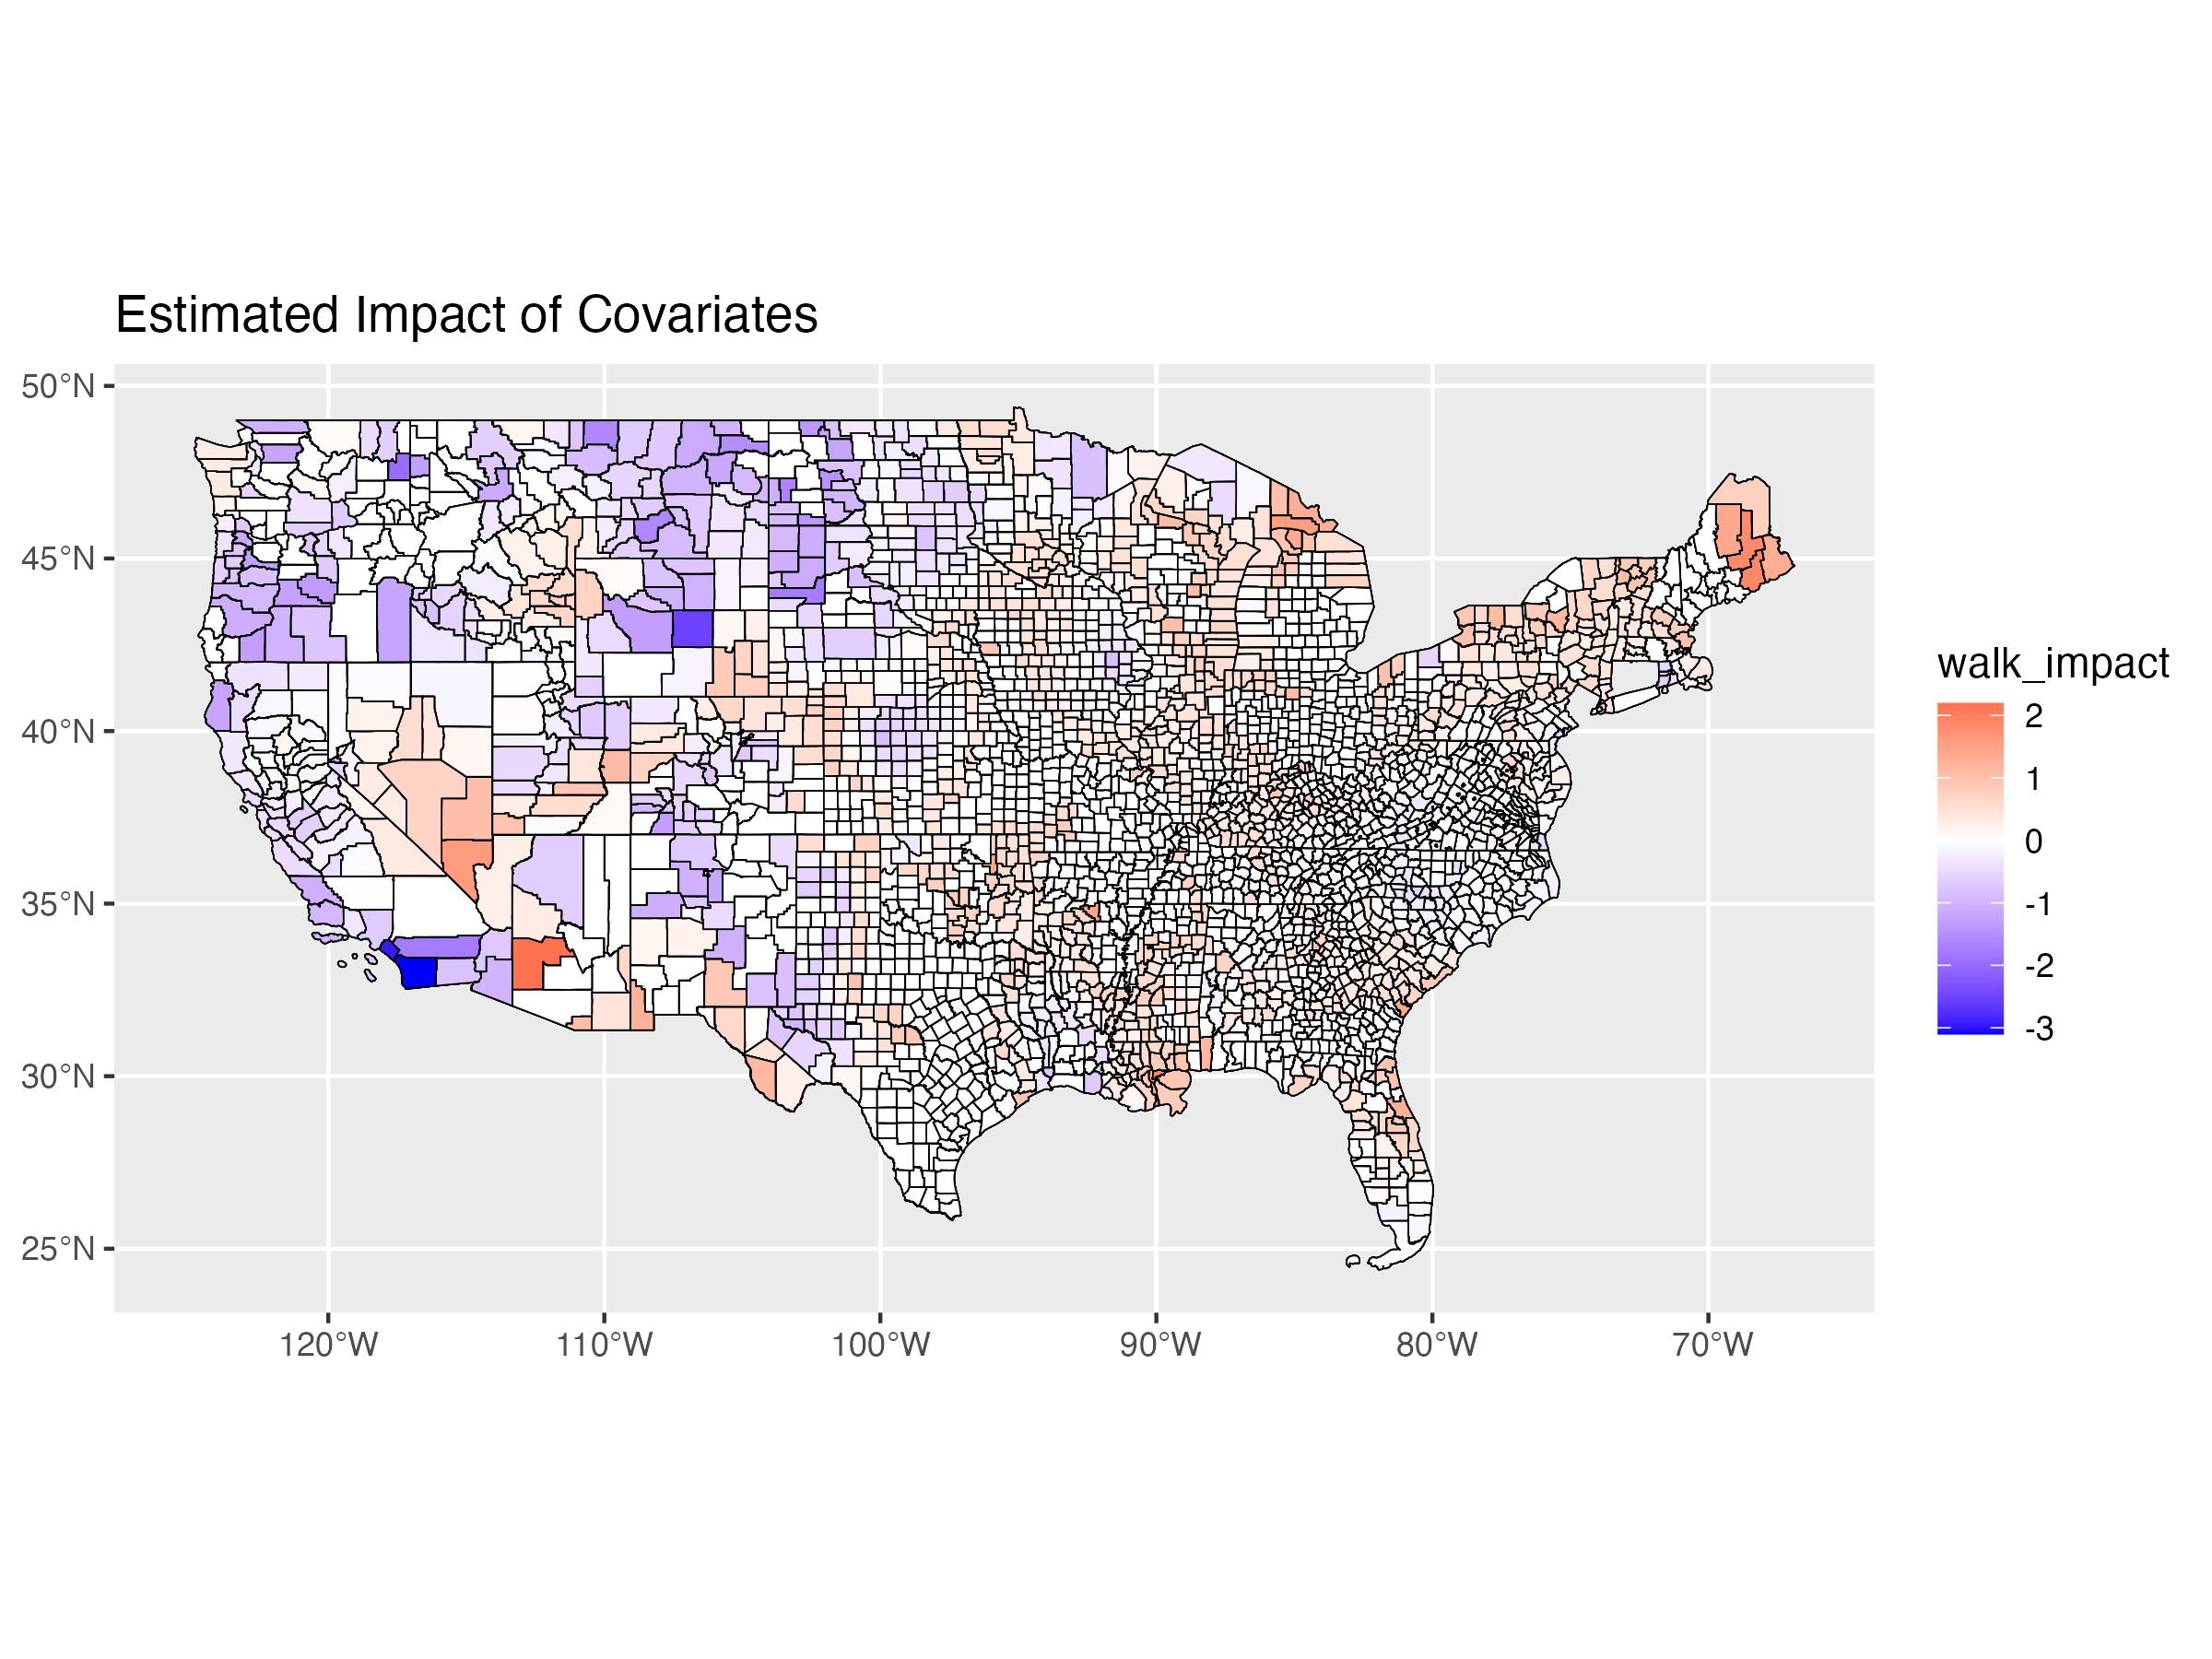
\includegraphics{impact_plot.png}

}

\caption{Impact of Walkability on Diabetes Prevalence}

\end{figure}%

When fitting the GWR model on our real-world data, we expected there to
be a consistent trend between walkability and diabetes prevalence across
the U.S. Accounting for walkability, multiple health risk factors,
temperature, income,etc, we expected there to be a consistent trend
between walkability and diabetes prevalence. However, from Figure 1
above, we can see that this is not the case. As seen in the West Coast,
Pacific North West, and the Mountainous Regions in the Northern part of
the U.S, there is a negative correlation between walkability and
diabetes prevalence. However, in the East Coast and Southern Regions of
the U.S there is a positive correlation between walkability and diabetes
prevalence. Ultimately, since there is a lack of consistency across the
U.S we believe that the walkability index score calculated by the CDC is
inaccurate and fails to account for certain additional factors to
explain the true impact of walkability on diabetes prevalence.

\begin{figure}[H]

{\centering 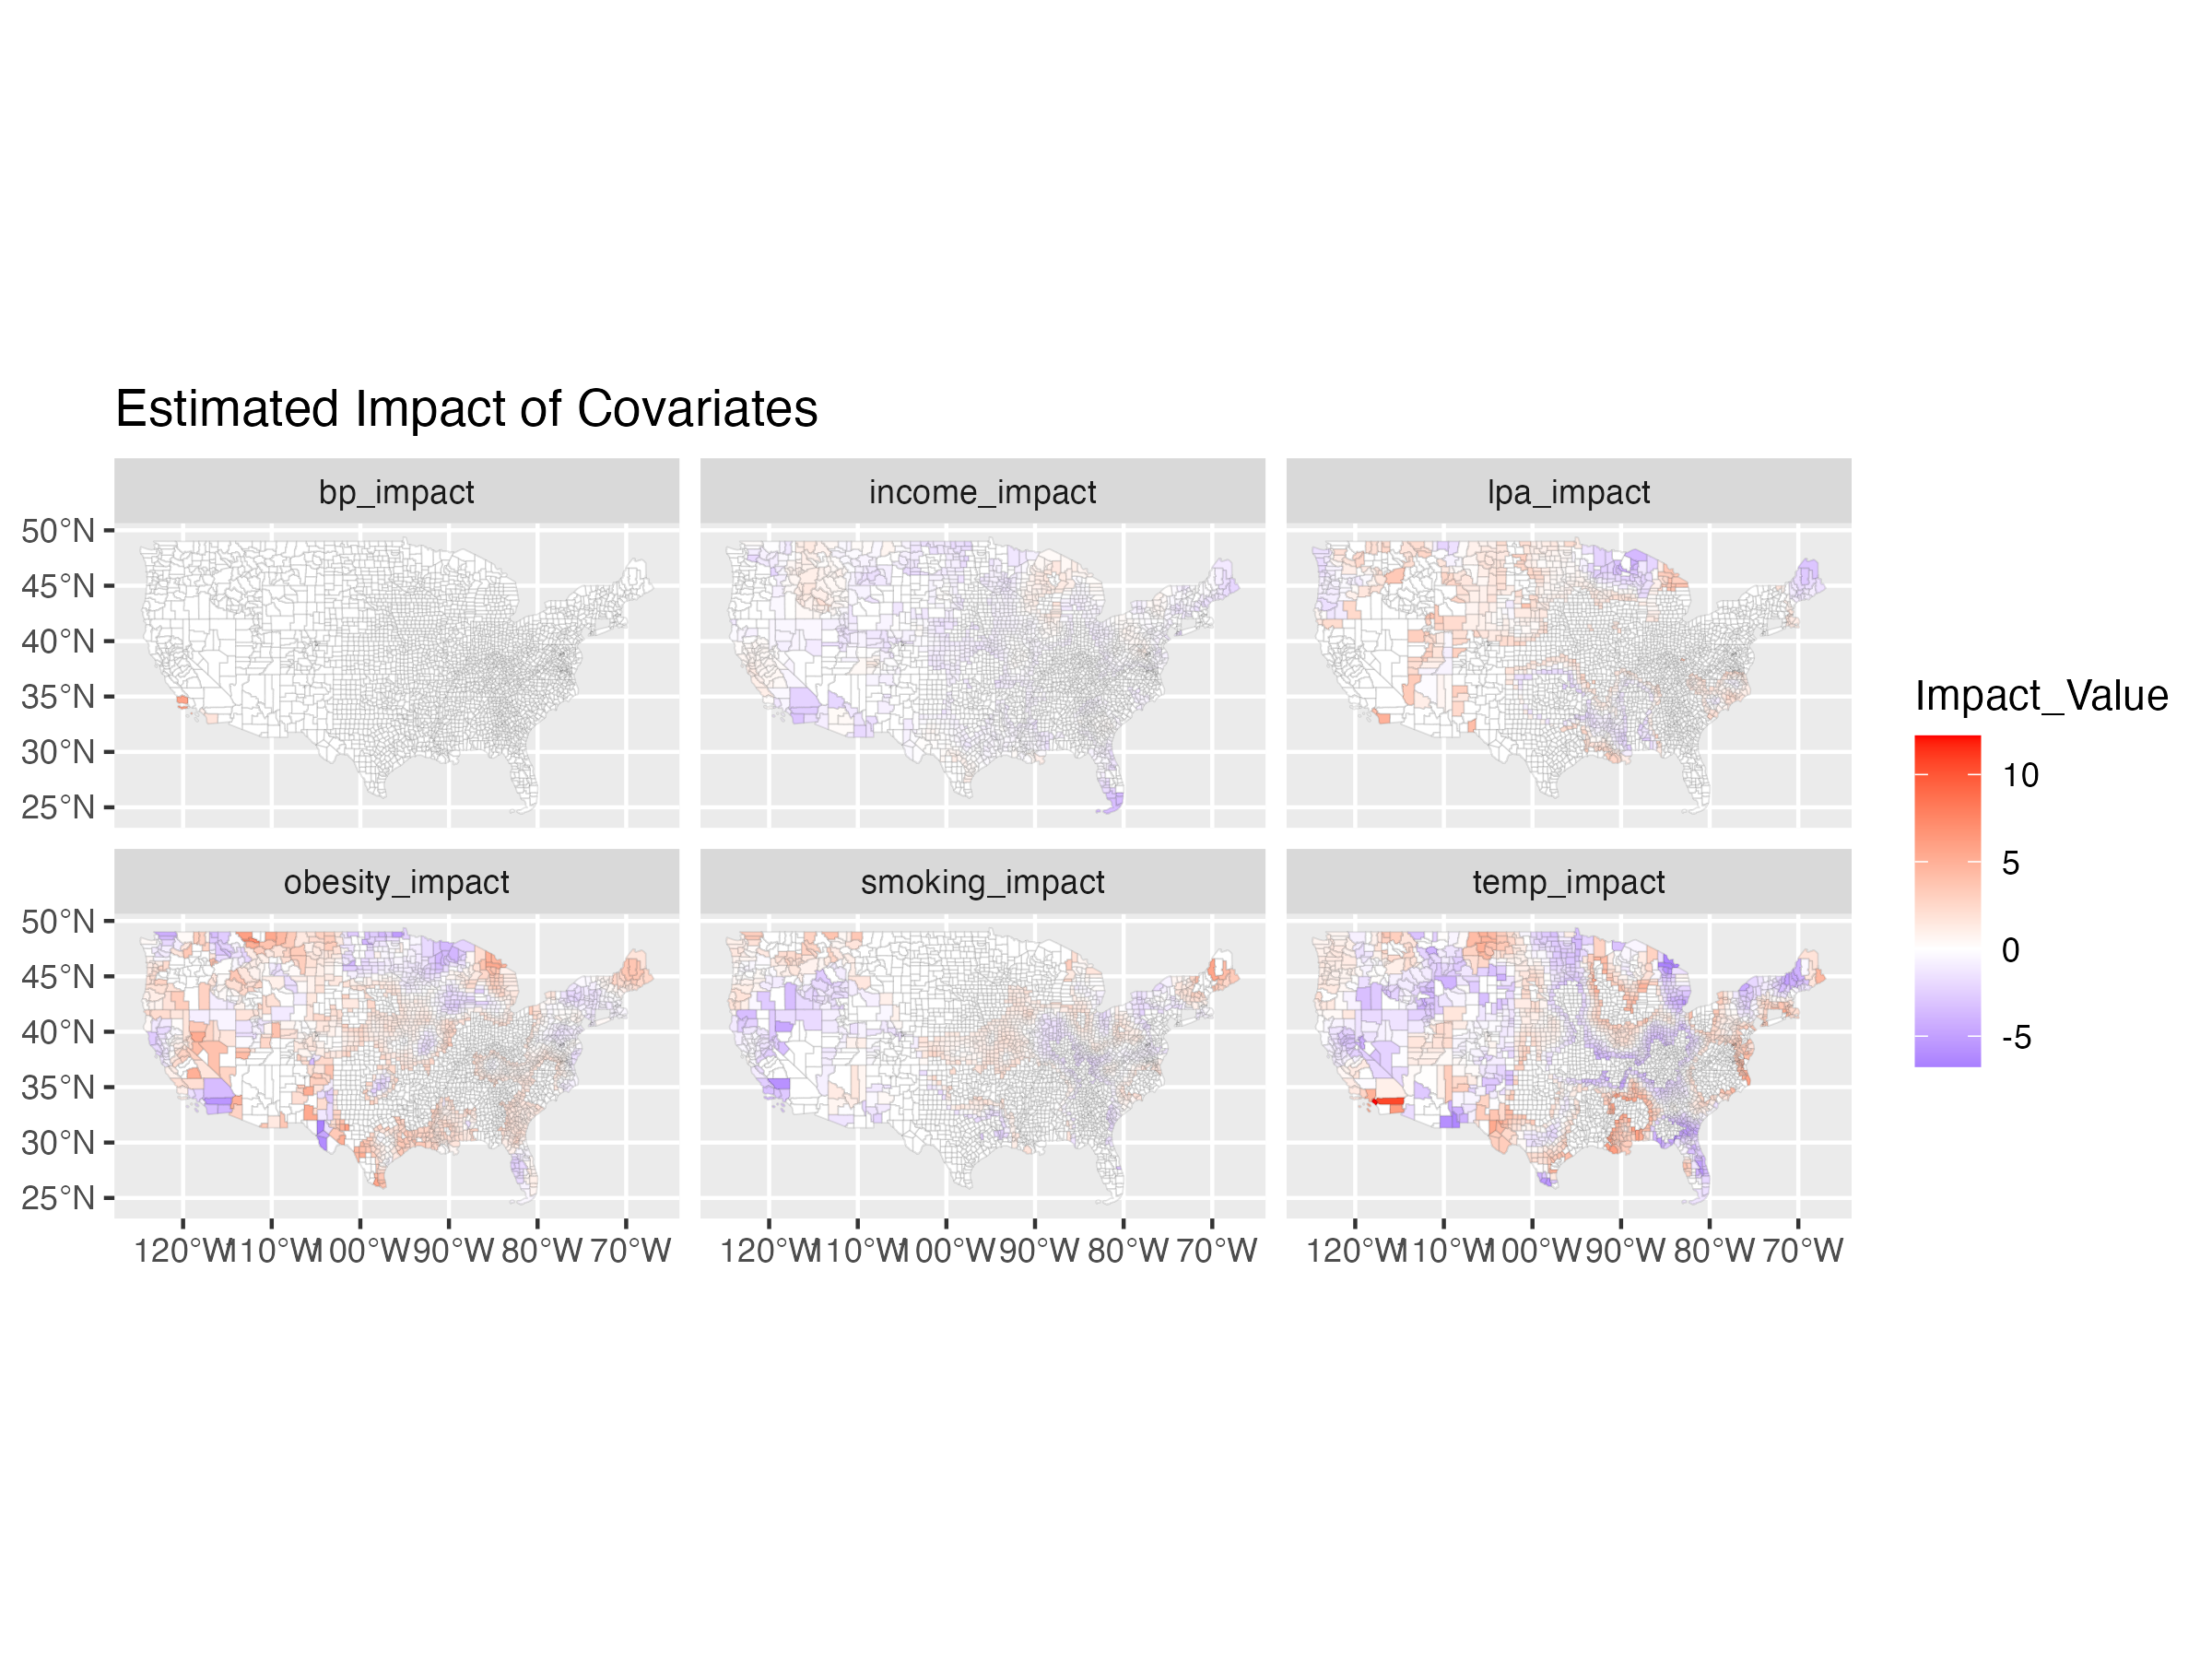
\includegraphics{facet_plot.png}

}

\caption{Impact of Covariates on Diabetes Prevalence}

\end{figure}%

\subsection{Validation}\label{validation-1}

\subsubsection{Monte Carlo Significance
Test}\label{monte-carlo-significance-test}

We first conducted a Monte-Carlo Significance Test to check for spatial
variation in each of our covariates. Table 3 below depicts the results
of our Monte-Carlo Significance Test. As we can see, the National
Walkability Index has a p-value of 0.45. This emphasizes that the
National Walkability Index is not significantly spatially varying. Thus,
if we were to model the National Walkability Index on a global scale, it
would not change our model's results much. This value further proves our
point that that the Walkability Index provided by the CDC may fail to
account for other essential factors that could further explain the
impact of walkability on diabetes prevalence.

\begin{longtable}[]{@{}lr@{}}
\caption{Results of Monte Carlo Simulation}\tabularnewline
\toprule\noalign{}
Covariates & P\_Value \\
\midrule\noalign{}
\endfirsthead
\toprule\noalign{}
Covariates & P\_Value \\
\midrule\noalign{}
\endhead
\bottomrule\noalign{}
\endlastfoot
Intercept & 0.39 \\
National Walkability Index & 0.35 \\
Obesity Prevalence & 0.01 \\
High Blood Pressure Prevalence & 0.00 \\
Low Physical Activity Prevalence & 0.00 \\
Current Smoking Prevalence & 0.00 \\
Median Household Income & 0.94 \\
Average Temperature & 0.00 \\
\end{longtable}

\subsubsection{Global Moran's I Test on
Residuals}\label{global-morans-i-test-on-residuals}

Next we conducted a Global Moran's I Test on the Residuals of our GWR
model to check for spatial autocorrelation. From the Global Moran's I
Test we obtained a Moran's 1 Statistic of 0.049. This indicates that
there is slight positive autocorrelation in our model. We expect this to
occur, as some of our covariates are similar in nature(eg. obesity,
smoking, high blood pressure,etc.). Ultimately, there is not significant
autocorrelation or an indication of high spatial dependence further
showing that our model is indeed accurate.

\begin{longtable}[]{@{}lr@{}}
\caption{Moran's I Test Results}\tabularnewline
\toprule\noalign{}
& Value \\
\midrule\noalign{}
\endfirsthead
\toprule\noalign{}
& Value \\
\midrule\noalign{}
\endhead
\bottomrule\noalign{}
\endlastfoot
Moran I statistic & 0.0448723 \\
Expectation & -0.0003249 \\
Variance & 0.0001135 \\
\end{longtable}

\subsubsection{Multicollinearity}\label{multicollinearity}

In addition, we examined if there was any significant multicollinearity
in our GWR model. We tested this by checking the Variance Inflation
Factor(VIF) for each of our covariates. For each of our covariates, none
of our values exceeded a VIF score of 13. This indicates that there is
not significant multicollinearity that poses an issue in our GWR model
indicating the validity of our model.

\subsubsection{Residuals}\label{residuals}

The residual plot in the Appendix shows a fairly evenly scattered
distribution of predicted values around zero, indicating a well-fitted
model. This further emphasizes the validity of our model.

In summary, the insights from our model, both from simulated and
real-world data, shed light on the complex interplay between
walkability, various risk factors, and diabetes prevalence across
different regions. The consistency between metrics obtained from our
simulation study and real data, coupled with the absence of
multicollinearity issues and spatial dependence , underscores the
reliability and validity of our findings, supporting the robustness of
our approach. Based on the results of the model along with the plots
that we made, we believe that the current formula used by the EPA and
other government agencies fail to consider many extraneous factors, and
the formula should be revised.

\section{Discussion}\label{discussion}

\subsection{Possible explanations for The Variation of Diabetes
Prevalence in Different
Regions}\label{possible-explanations-for-the-variation-of-diabetes-prevalence-in-different-regions}

The correlation between walkability and diabetes prevalence in the South
can be attributed to various factors, with higher temperatures emerging
as a key consideration. In warmer climates, such as those prevalent in
the South, the positive relationship between walkability and diabetes
may be influenced by people spending more time indoors to avoid the
heat. This reduction in outdoor activity diminishes walkability and
could potentially contribute to higher diabetes rates.Conversely, in
colder regions like the west coast and the Pacific Northwest, the impact
of walkability on diabetes prevalence appears to be negative, as
depicted in the plot. This suggests that regional differences, including
climate variations, play a significant role in shaping the relationship
between walkability and diabetes. Moreover, the analysis identified
various additional risk factors, notably health-related ones,
contributing to elevated diabetes prevalence nationwide. From the facet
plot depicted below, factors like smoking and obesity showed clear
associations with higher rates of diabetes, as expected given their
impact on overall health and predisposition to chronic conditions like
diabetes.

\subsection{Revisiting the EPA's Walkability Index in Light of Regional
Variations}\label{revisiting-the-epas-walkability-index-in-light-of-regional-variations}

Our analysis shows that the walkability index, as formulated by the EPA,
does not consistently predict diabetes outcomes across different U.S.
regions. This finding reflects the challenges mentioned in the
``National Walkability Index User Guide and Methodology,'' where
variables like intersection density and land use diversity may not
sufficiently capture regional factors that influence health outcomes.The
related work ``Development of an objectively measured walkability index
for the Netherlands'' suggests that walkability assessments must use
local urban layouts and societal norms to enhance their relevance and
accuracy. Taking this into account, our study proposes that additional
variables specific to regional characteristics in the U.S. should be
considered to improve the predictive power of the walkability index
concerning diabetes prevalence.

\subsection{Aligning Methodological Approaches with Urban Health
Outcomes}\label{aligning-methodological-approaches-with-urban-health-outcomes}

The inconsistencies we observed in walkability's impact on diabetes
prevalence across different U.S. regions highlight the need for a more
nuanced approach to walkability assessments, as suggested by the diverse
methodologies mention in ``Planning and Design Support Tools for
Walkability.'' This source suggests using tools that adapt to different
city environments, emphasizing the need to customize walkability indices
to both physical and social aspects of cities. In addition, the study
``Spatial Pattern of the Walkability Index, Walk Score, and Walk Score
Modification for Elderly'' shows the importance of adapting indices to
specific demographic needs, such as adjusting for elderly populations.
Similarly, our findings advocate for the adaptation of walkability
indices to better address the health implications of walkability in
regions with different urban dynamics and demographic profiles.

\subsection{Enhancing Walkability Indices through Tailored
Assessments}\label{enhancing-walkability-indices-through-tailored-assessments}

Our research further confirms the belief from ``Development of a
Child-Focused Walkability Index'' that walkability assessments should
consider demographic-specific needs. Just as traffic volume and sidewalk
presence are crucial for assessing children's mobility in urban areas,
our results suggest that factors like community health services access,
food landscapes, and recreational spaces might be significant predictors
of diabetes prevalence related to walkability. This perspective aligns
with our observation that the existing walkability indices may overlook
critical elements that influence health outcomes in varied urban
settings.

\subsection{Proposed Modifications to Current Walkability
Calculations}\label{proposed-modifications-to-current-walkability-calculations}

Given the regional anomalies noted in our study, we propose several
modifications to the current methods of calculating the walkability
index. These include incorporating health-related facilities access and
community socio-economic status to provide a more comprehensive method
of how walkability influences diabetes prevalence. This approach is
inspired by the modifications discussed in the ``Spatial Pattern of the
Walkability Index, Walk Score and Walk Score Modification for Elderly,''
which adapted traditional metrics to better suit elderly residents by
considering their specific mobility and access needs.

\subsubsection{Conclusion}\label{conclusion}

In conclusion, our study shows that we need to improve the walkability
index by including more detailed factors that consider both the physical
layout and the social and economic conditions of neighborhoods. By
adding these details to walkability assessments, city planners and
health officials can better understand how city design affects public
health, and work more effectively to reduce health risks related to
areas that are hard to walk in. Our research points out the complex ways
in which city planning and public health are connected, suggesting that
city planning should take a more detailed and specific approach that
meets the diverse needs of different communities. Looking ahead, more
studies are needed that follow how changes in city planning affect
public health over time. This will provide solid evidence to guide
decisions in making cities healthier and more walkable.

\newpage{}

\section{Appendix}\label{appendix}

\begin{figure}[H]

{\centering 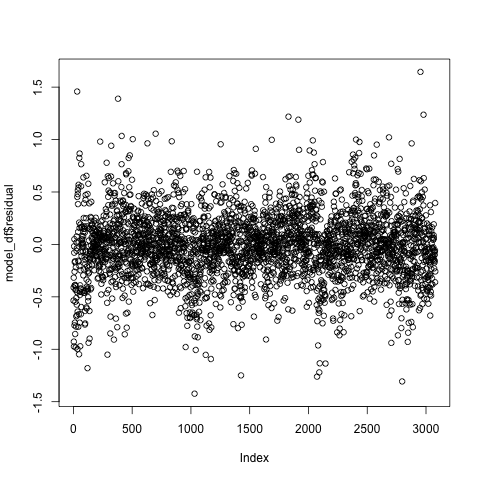
\includegraphics{residual_plot.png}

}

\caption{Resdiual Plot of GWR Model}

\end{figure}%

\newpage{}

\section{References}\label{references}

\begin{itemize}
\tightlist
\item
  Smith, J., et al.~(2020). Do the risk factors for type 2 diabetes
  mellitus vary by location? A spatial analysis of health insurance
  claims in Northeastern Germany using kernel density estimation and
  geographically weighted regression. \emph{Journal of Public Health
  Research}.
\item
  Jones, D., \& Taylor, B. (2019). Spatial Analysis of Incidence of
  Diagnosed Type 2 Diabetes Mellitus and Its Association With Obesity
  and Physical Inactivity. \emph{Journal of Clinical Epidemiology}.
\item
  G. Xu et al., ``Prevalence of diagnosed type 1 and type 2 diabetes
  among US adults in 2016 and 2017: population based study,''
\item
  M. I. Creatore et al., ``Association of Neighborhood Walkability With
  Change in Overweight, Obesity, and Diabetes''
\item
  R. H. Glazier et al., ``Density, Destinations or Both? A Comparison of
  Measures of Walkability in Relation to Transportation Behaviors,
  Obesity and Diabetes in Toronto, Canada,'' PLoS ONE, vol.~9, no. 1,
  p.~e85295, Jan.~2014, doi: 10.1371/journal.pone.0085295.
\item
  M. A. Lazar, ``How Obesity Causes Diabetes: Not a Tall Tale,''
  Science, vol.~307, no. 5708, pp.~373--375, Jan.~2005, doi:
  10.1126/science.1104342.
\item
  C. Brunsdon, A. S. Fotheringham, and M. E. Charlton, ``Geographically
  Weighted Regression: A Method for Exploring Spatial Nonstationarity,''
  Geographical Analysis, vol.~28, no. 4, pp.~281--298, Oct.~1996, doi:
  10.1111/j.1538-4632.1996.tb00936.x.
\item
  Byrne, Graeme \& Charlton, Martin \& Fotheringham, Alexander. (2009).
  Multiple Dependent Hypothesis Tests in Geographically Weighted
  Regression.
\item
  Bureau, US Census. ``Small Area Income and Poverty Estimates (SAIPE)
  Program.'' Census.Gov, 1 July 2022,
  www.census.gov/programs-surveys/saipe.html.
\item
  U.S. Environmental Protection Agency, ``National Walkability Index
  User Guide and Methodology.'' Available:
  \href{https://www.epa.gov/smartgrowth/national-walkability-index-user-guide-and-methodology}{EPA
  Walkability Index User Guide and Methodology}
\item
  M. Poelman, ``Development of an objectively measured walkability index
  for the Netherlands,'' International Journal of Behavioral Nutrition
  and Physical Activity, 2022. Available:
  \href{https://ijbnpa.biomedcentral.com/articles/10.1186/s12966-022-01270-8}{Development
  of an objectively measured walkability index for the Netherlands}
\item
  R. H. Glazier et al., ``Planning and Design Support Tools for
  Walkability,'' Sustainability, vol.~12, no. 11, May 2020. Available:
  \href{https://www.mdpi.com/2071-1050/12/11/4405}{Planning and Design
  Support Tools for Walkability}
\item
  V. Schuurman et al., ``Spatial Pattern of the Walkability Index, Walk
  Score and Walk Score Modification for Elderly,'' International Journal
  of Health Geographics, vol.~11, no. 5, 2020. Available:
  \href{https://www.mdpi.com/2220-9964/11/5/279}{Spatial Pattern of the
  Walkability Index, Walk Score and Walk Score Modification for Elderly}
\item
  L. Giles-Corti et al., ``Development of a Child-Focused Walkability
  Index,'' International Journal of Health Geographics, vol.~12, 2013.
  Available:
  \href{https://ij-healthgeographics.biomedcentral.com/articles/10.1186/1476-072X-12-61}{Development
  of a Child-Focused Walkability Index}
\item
  A. H. Mokdad et al., ``Prevalence of Obesity, Diabetes, and
  Obesity-Related Health Risk Factors, 2001,'' JAMA, vol.~289, no. 1,
  p.~76, Jan.~2003, doi: 10.1001/jama.289.1.76.
\item
  J. Chapman, E. Fox, W. Bachman, L. Frank, J. Thomas, and A. Rourk
  Reyes, ``Smart Location Database Technical Documentation and User
  Guide Version 3.0,'' Jun.~2021, {[}Online{]}. Available:
  \href{https://www.epa.gov/system/files/documents/2023-10/epa_sld_3.0_technicaldocumentationuserguide_may2021_0.pdf}{EPA
  Smart Location Database}
\item
  I. Gollini, B. Lu, M. Charlton, C. Brunsdon, and P. Harris, ``GWmodel:
  An R Package for Exploring Spatial Heterogeneity Using Geographically
  Weighted Models,'' J. Stat. Soft., vol.~63, no. 17, 2015, doi:
  10.18637/jss.v063.i17.
\item
  ``Places: Census Tract Data (GIS Friendly Format), 2021 Release.''
  Centers for Disease Control and Prevention, Centers for Disease
  Control and Prevention, 2023,
  data.cdc.gov/500-Cities-Places/PLACES-Census-Tract-Data-GIS-Friendly-Format-2021-/mb5y-ytti/about\_data.
\item
  Gilbert, Mark. ``Heat Health Census Tracts.'' GIS For Racial Equity,
  gis-for-racialequity.hub.arcgis.com/datasets/climatesolutions::heat-health-census-tracts/about.
  Accessed 3 May 2024.
\item
  S. Gebel, M. Rapp, A. Voigtländer, A. Schneider, R. Döring, and S.
  Karrasch, ``Walkability and its association with prevalent and
  incident diabetes in a pooled sample from five German cohorts,'' BMC
  Endocrine Disorders, vol.~19, no. 101, 2019, doi:
  10.1186/s12902-019-0485-x
\item
  J. Booth, J. R. Parks, and T. L. Frost, ``Neighborhood walkability and
  pre-diabetes incidence in a multiethnic population,'' BMJ Open
  Diabetes Research \& Care, vol.~8, no. 1, 2020, doi:
  10.1136/bmjdrc-2020-001533
\end{itemize}



\end{document}
